\documentclass[11pt,a4paper]{article}

% ---- Idioma y tipografía
\usepackage[spanish, es-noquoting, es-noshorthands]{babel}
\usepackage[T1]{fontenc}
\usepackage[utf8]{inputenc} % eliminar si usas XeLaTeX/LuaLaTeX
\usepackage{lmodern}
\usepackage{microtype}

% ---- Márgenes y diseño
\usepackage[a4paper,margin=2.5cm]{geometry}
\usepackage{parskip}

% ---- Enlaces
\usepackage[hidelinks]{hyperref}
\usepackage{bookmark}

% ---- Cabeceras y pies
\usepackage{fancyhdr}
\pagestyle{fancy}
\fancyhf{}
\renewcommand{\headrulewidth}{0.4pt}
\lhead{\textsc{\asignatura}}
\chead{\textbf{\tema}}
\rhead{\clase\;|\; \fecha}
\cfoot{\thepage}

% ---- Listas y símbolos
\usepackage{enumitem}
\setlist{itemsep=0.3em, topsep=0.5em}

% ---- Iconos y color
\usepackage{fontawesome5}
\usepackage{xcolor}
\usepackage[most]{tcolorbox}
\tcbuselibrary{breakable,skins}

% ---- Colores propios
\definecolor{uniPrimary}{HTML}{0A7AC3}
\definecolor{uniSoft}{HTML}{E9F4FB}
\definecolor{uniAccent}{HTML}{F5B700}
\definecolor{uniOK}{HTML}{2E7D32}
\definecolor{uniWarn}{HTML}{C62828}

% ---- Metadatos reutilizables
\newcommand{\asignatura}{Seguridad de Sistemas Informáticos}
\newcommand{\tema}{Tema 1 — Introducción}
\newcommand{\clase}{Clase 1}
\newcommand{\fecha}{\today}

% ---- Estética de secciones
\usepackage{titlesec}
\titleformat{\section}{\Large\bfseries\color{uniPrimary}}{\thesection}{0.6em}{}
\titleformat{\subsection}{\large\bfseries}{\thesubsection}{0.5em}{}
\titleformat{\subsubsection}{\bfseries}{\thesubsubsection}{0.5em}{}

% ---- Cajas reutilizables
\tcbset{
    commonstyle/.style={
        enhanced, breakable,
        left=8pt,right=8pt,top=8pt,bottom=8pt,
        boxrule=0.8pt,
        fonttitle=\bfseries
    }
}

\newtcolorbox{ObjetivosBox}[1][]{
    commonstyle,
    title={\faBullseye\; Índice},
    colback=uniSoft, colframe=uniPrimary,#1
}

\newtcolorbox{DefBox}[1][]{
    commonstyle,
    title={\faBook\; Definición},
    colback=white, colframe=uniAccent,#1
}

\newtcolorbox{NotaBox}[1][]{
    commonstyle,
    title={\faStickyNote\; Nota},
    colback=white, colframe=uniPrimary,#1
}

\newtcolorbox{RecordatorioBox}[1][]{
    commonstyle,
    title={\faBell\; Recordatorio},
    colback=uniAccent!15, colframe=uniAccent,#1
}

\newtcolorbox{ChecklistBox}[1][]{
    commonstyle,
    title={\faTasks\; Tareas / Checklist},
    colback=white, colframe=uniPrimary,#1
}

\newtcolorbox{ResumenBox}[1][]{
    commonstyle,
    title={\faHighlighter\; Resumen rápido (5 líneas)},
    colback=uniSoft, colframe=uniPrimary,#1
}

\newtcolorbox{VocabBox}[1][]{
    commonstyle,
    title={\faLanguage\; Vocabulario clave},
    colback=white, colframe=uniPrimary,#1
}

% =========================================================
\begin{document}

    % ---- Cabecera de ficha de clase
    {\large \textbf{\asignatura} \;—\; \textbf{\tema} \hfill \textit{\clase, \fecha}}\\[0.6em]
    \faUser\; Alumno/a: Alberto Díaz Maroto Ortiz\hfill
    \faChalkboardTeacher\; Profesor/a: Sebastián Reyes

    \vspace{1em}
    \tableofcontents
    \vspace{1em}

    \begin{NotaBox}
        Apuntes \textit{resumidos y traducidos} del capítulo 1 (\textit{Overview}) de \textbf{Computer Security: Principles and Practice}. Referencias conceptuales: glosario NISTIR~7298 y FIPS~200. :contentReference[oaicite:1]{index=1}
    \end{NotaBox}

    \begin{ObjetivosBox}
        \begin{itemize}
            \item Definir seguridad informática y la tríada \textbf{CIA}.
            \item Identificar activos, amenazas, ataques y contramedidas.
            \item Resumir requisitos funcionales (FIPS~200) y principios de diseño.
            \item Explicar \textit{superficie de ataque}, \textit{defensa en profundidad} y árboles de ataque.
            \item Esbozar política, implementación, \textit{assurance} y evaluación.
        \end{itemize}
    \end{ObjetivosBox}

    \section{Conceptos básicos}
    \begin{DefBox}
        \textbf{Seguridad informática:} Medidas y controles para asegurar \textbf{confidencialidad}, \textbf{integridad} y \textbf{disponibilidad} de los activos del sistema (HW, SW, firmware, datos en proceso/almacenamiento/transmisión). \textit{(NISTIR~7298)}. :contentReference[oaicite:3]{index=3}
    \end{DefBox}

    \subsection{Tríada CIA y niveles de impacto}
    \begin{itemize}
        \item \textbf{Confidencialidad:} \textbf{acceso/divulgación sólo a sujetos autorizados}. No se puede divulgar.
        \item \textbf{Integridad:} \textbf{protección frente a modificación o destrucción indebida}; autenticidad y no repudio.
        \item \textbf{Disponibilidad:} \textbf{acceso oportuno a la información/servicios}. Ininterrupción mínima.
        \item \textbf{Impacto:} \textbf{bajo, moderado, alto} según el efecto adverso esperado en la organización o individuos.
    \end{itemize}

    \section{Retos de la seguridad}
    \begin{itemize}
        \item No es trivial: hay que anticipar ataques y ubicar bien los controles.
        \item Requiere \textit{secretos} (claves, credenciales): creación, distribución y protección.
        \item Los procedimientos suelen ser complejos y dificiles de entender.
        \item El atacante necesita una sola vulnerabilidad; el defensor debe cerrar todas.
        \item Suele añadirse tarde; demanda monitoreo continuo.
        \item Percepción de “poca utilidad” hasta que ocurre un incidente; fricción con la usabilidad.
    \end{itemize}

    \section{Activos, amenazas y ataques}
    \subsection{Activos y vulnerabilidades}
    \begin{itemize}
        \item \textbf{Activos:} hardware, software, datos, comunicaciones/redes.
        \item \textbf{Vulnerabilidades:} pérdida de integridad (\textit{corruption}), confidencialidad (\textit{leakage}) o disponibilidad (\textit{unavailability}). :contentReference[oaicite:6]{index=6}
    \end{itemize}

    \subsection{Amenazas y ataques}
    \begin{itemize}
        \item \textbf{Amenaza:} circunstancia con potencial de dañar un activo explotando una debilidad.
        \item \textbf{Ataques:} \emph{pasivos} (escucha, análisis de tráfico) vs. \emph{activos} (replay, suplantación, modificación, DoS); origen \emph{interno} o \emph{externo}. :contentReference[oaicite:7]{index=7}
    \end{itemize}

    \subsection{Contramedidas}
    \begin{itemize}
        \item \textbf{Prevenir} \(\rightarrow\) \textbf{Detectar} \(\rightarrow\) \textbf{Recuperar}; minimizar el riesgo residual (toda defensa puede introducir nuevas debilidades). :contentReference[oaicite:8]{index=8}
    \end{itemize}

    \section{Consecuencias típicas y acciones de ataque}
    \begin{itemize}
        \item \textbf{Divulgación no autorizada:} exposición, interceptación, inferencia, intrusión.
        \item \textbf{Engaño:} suplantación, falsificación, repudio.
        \item \textbf{Disrupción:} incapacitación, corrupción, obstrucción.
        \item \textbf{Usurpación:} apropiación de recursos, uso indebido. \textit{(basado en RFC 4949)}. :contentReference[oaicite:9]{index=9}
    \end{itemize}

    \section{Requisitos de seguridad (síntesis FIPS~200)}
    \begin{itemize}[leftmargin=1.2em]
        \item Control de acceso; Concienciación y formación; Auditoría y \textit{accountability}.
        \item Certificación/evaluaciones; Gestión de configuración; Continuidad/contingencia.
        \item Identificación y autenticación; Respuesta a incidentes; Mantenimiento.
        \item Protección de medios; Protección física/ambiental; Planificación.
        \item Seguridad de personal; Gestión de riesgos.
        \item Adquisición de sistemas/servicios; Protección de sistemas y comunicaciones.
        \item Integridad de sistema e información. :contentReference[oaicite:10]{index=10}
    \end{itemize}

    \section{Principios de diseño de seguridad}
    \begin{itemize}
        \item Economía del mecanismo; \textit{Fail-safe defaults}; Mediación completa; Diseño abierto.
        \item Separación y \textbf{mínimo} privilegio; Mecanismo común mínimo; Aceptabilidad psicológica.
        \item Aislamiento, encapsulación, modularidad, \textit{layering}, sorpresa mínima. :contentReference[oaicite:11]{index=11}
    \end{itemize}

    \section{Superficie de ataque y árboles de ataque}
    \subsection{Superficie de ataque}
    \begin{itemize}
        \item Conjunto de vulnerabilidades alcanzables/explotables: puertos y servicios, código que procesa entradas, interfaces/SQL/webforms, formatos de intercambio, y el factor humano (ingeniería social). :contentReference[oaicite:12]{index=12}
    \end{itemize}
    \subsection{Categorías}
    \begin{itemize}
        \item \textbf{Red}, \textbf{software} y \textbf{humana}. Relacionar con \textit{defensa en profundidad}. :contentReference[oaicite:13]{index=13}
    \end{itemize}
    \subsection{Árboles de ataque}
    \begin{itemize}
        \item Modelo jerárquico para descomponer objetivos del atacante (ej.: autenticación bancaria) y evaluar controles. :contentReference[oaicite:14]{index=14}
    \end{itemize}

    \section{Estrategia de seguridad}
    \begin{itemize}
        \item \textbf{Política:} reglas prácticas para proteger recursos críticos.
        \item \textbf{Implementación:} prevención, detección, respuesta y recuperación.
        \item \textbf{Assurance:} confianza en que el sistema hace cumplir la política.
        \item \textbf{Evaluación:} examen y pruebas frente a criterios definidos.
    \end{itemize}

    \section{Organismos y normas}
    \begin{itemize}
        \item \textbf{NIST}, \textbf{ISOC/IETF}, \textbf{ITU-T}, \textbf{ISO}. Cobertura: buenas prácticas de gestión y arquitectura de controles. :contentReference[oaicite:16]{index=16}
    \end{itemize}

    \begin{VocabBox}
        \textbf{Adversario:} agente con intención/capacidad de causar daño. \;
        \textbf{Riesgo:} función de impacto y probabilidad. \;
        \textbf{Política de seguridad:} criterios que regulan servicios y comportamientos. \;
        \textbf{Activo:} recurso valioso (sistema, datos, personal, instalaciones). \;
        \textbf{Amenaza:} evento con potencial daño. \;
        \textbf{Vulnerabilidad:} debilidad explotable. :contentReference[oaicite:17]{index=17}
    \end{VocabBox}

    \begin{ResumenBox}
        Seguridad protege \textbf{CIA} frente a amenazas que explotan vulnerabilidades en activos.
        Los ataques pueden ser pasivos/activos y generar divulgación, engaño, disrupción o usurpación.
        Se mitigan con contramedidas y un marco de requisitos (FIPS~200) y principios de diseño.
        La \textit{superficie de ataque} guía la \textit{defensa en profundidad}; los árboles de ataque ayudan a analizar objetivos.
        La estrategia combina política, implementación, \textit{assurance} y evaluación, alineada con estándares NIST/ISOC/ITU/ISO. :contentReference[oaicite:18]{index=18}
    \end{ResumenBox}

    \section{Servicios de seguridad}
    \begin{itemize}
        \item \textbf{Autenticación:} Garantiza que la identidad de usuarios, entidades o sistemas sea verificada antes de conceder acceso.
        \item \textbf{Control de acceso:} Restringe el acceso a recursos y servicios sólo a sujetos autorizados, según políticas definidas.
        \item \textbf{Confidencialidad de datos:} Protege la información frente a accesos o divulgaciones no autorizadas, normalmente mediante cifrado.
        \item \textbf{Integridad de datos:} Asegura que la información no sea alterada o destruida de forma no autorizada.
        \item \textbf{No repudio:} Impide que una entidad niegue la autoría de una acción o comunicación previamente realizada.
        \item \textbf{Disponibilidad:} Garantiza que los sistemas y datos estén accesibles y operativos cuando se necesiten.
    \end{itemize}

    No son lo mismo los mecanismos de seguridad que los servicios de seguridad. Por ejemplo, el cifrado es un mecanismo que proporciona el servicio de confidencialidad.
    Los mecanismos son implementaciones tecnicas que satisfacen los requisitos de los servicios de seguridad.

    \subsection{Autenticación}
    La autenticación puede referirse tanto a entidades como a datos:

    \begin{itemize}
        \item \textbf{Autenticación de entidades:} Verifica la identidad de dos entidades que se comunican en el mismo nivel y usando el mismo protocolo. Por ejemplo, el chat de Teams autentica a los usuarios que participan en la conversación.
        \item \textbf{Autenticación de origen de datos:} Corrobora la fuente de una unidad de datos, asegurando que proviene de quien dice ser (por ejemplo, mediante firma digital). No protege contra duplicados ni modificaciones, solo garantiza el origen. Es común en aplicaciones asíncronas como el correo electrónico.
    \end{itemize}

    \subsection{Control de acceso}
    El control de acceso regula qué usuarios o entidades pueden acceder a determinados recursos o servicios, y bajo qué condiciones. Se basa en políticas que definen permisos y restricciones, y puede implementarse mediante listas de control de acceso (ACL), roles, o atributos. El objetivo es asegurar que sólo los sujetos autorizados puedan realizar operaciones específicas sobre los objetos protegidos.

    \subsection{Confidencialidad de datos}
    La confidencialidad de datos busca evitar que la información sea revelada a personas o sistemas no autorizados. Se pueden distinguir dos aspectos principales:

    \begin{itemize}
        \item \textbf{Protección contra ataques pasivos:} Consiste en impedir que un atacante pueda leer el contenido de los mensajes transmitidos, por ejemplo, mediante cifrado de datos. Así, aunque los datos sean interceptados, no podrán ser interpretados sin la clave adecuada.
        \item \textbf{Protección contra análisis de tráfico:} Va más allá del cifrado, intentando ocultar patrones de comunicación, volúmenes, frecuencia o duración de las transmisiones. Técnicas como el envío de mensajes de relleno o el enmascaramiento de la longitud de los paquetes dificultan que un atacante deduzca información sensible a partir del tráfico observado.
    \end{itemize}

    \subsection{Integridad de datos}
    La integridad de datos garantiza que la información no sea modificada, insertada, eliminada o reordenada de forma no autorizada durante la transmisión o almacenamiento. Existen dos modalidades:

    \begin{itemize}
        \item \textbf{Integridad orientada a conexión:} Asegura que, en una comunicación continua (como HTTP), los mensajes lleguen sin duplicados, inserciones, reordenaciones o repeticiones. Se protege la secuencia y unicidad de los mensajes intercambiados.
        \item \textbf{Integridad sin conexión:} Aplica a protocolos sin sesión establecida (como UDP), donde se protege cada mensaje individualmente contra modificaciones, pero no se garantiza el orden ni la unicidad. El objetivo principal es detectar cualquier alteración en el contenido del mensaje.
    \end{itemize}

    \subsection{No repudio}
    El no repudio asegura que el remitente no pueda negar haber enviado un mensaje y el receptor no pueda negar haberlo recibido, normalmente mediante firmas digitales o acuses de recibo firmados.

    \subsection{Disponibilidad}
    La disponibilidad asegura que sistemas y datos estén accesibles cuando se necesiten. Se protege mediante tolerancia a fallos, redundancia y gestión de recursos, y se enfrenta a amenazas como los ataques de denegación de servicio (DoS).

    \section{Mecanismos de seguridad}

    Los mecanismos de seguridad son técnicas, procedimientos o dispositivos que implementan los servicios de seguridad y protegen los sistemas frente a amenazas específicas. Entre los mecanismos más relevantes se encuentran:

    \begin{itemize}
        \item \textbf{Algoritmos criptográficos:} Transforma la información para que sólo pueda ser leída por quienes posean la clave adecuada, protegiendo la confidencialidad y, en algunos casos, la integridad.
        \begin{itemize}
            \item \textbf{Keyless:} Hash (SHA-2, SHA-3) para integridad, PRNG para aleatoriedad.
            \item \textbf{Single Key:} MAC y cifrado simétrico (AES, DES).
            \item \textbf{Two Key:} Autenticación de usuario, firma digital (RSA, ECDSA), cifrado asimétrico.
        \end{itemize}

        \item \textbf{Cifrado:} Transforma la información para que sólo pueda ser leída por quienes posean la clave adecuada, protegiendo la confidencialidad y, en algunos casos, la integridad.
        \item \textbf{Firmas digitales:} Permiten verificar la autenticidad e integridad de los datos, y proporcionan no repudio.
        \item \textbf{Intercambio de autenticación:} Protocolos para verificar identidades y, opcionalmente, establecer claves de sesión de forma segura (por ejemplo, desafío-respuesta o autenticación mutua).
        \item \textbf{Relleno de tráfico:} Inserción de datos o mensajes de relleno para ocultar patrones de volumen, frecuencia y longitud frente al análisis de tráfico.
        \item \textbf{Control de enrutamiento:} Selección o restricción de rutas para que los datos circulen por caminos confiables, evitando nodos o redes no autorizadas.
        \item \textbf{Notorización:} Uso de un tercero de confianza que certifica la existencia, envío o recepción de datos/eventos en un instante, aportando evidencia para no repudio.
        \item \textbf{Control de acceso:} Mecanismos que aplican políticas para limitar operaciones de sujetos sobre objetos (basados en listas, roles o atributos).
    \end{itemize}
    \section{Principios fundamentales de diseño de seguridad}

    \begin{NotaBox}
        Resumen (Saltzer \& Schroeder): economía del mecanismo, \textit{fail-safe defaults} y mediación completa.
    \end{NotaBox}

    \begin{itemize}
        \item \textbf{Economía del mecanismo:} simplicidad y tamaño mínimo para reducir errores y superficie.
        \item \textbf{Fail-safe defaults:} negar por defecto y fallar cerrando; configuración inicial segura.
        \item \textbf{Mediación completa:} autorizar cada acceso; sin bypass; revocaciones efectivas.
        \item \textbf{Diseño abierto:} no depender del secreto del diseño; fortaleza en claves y estándares abiertos.
        \item \textbf{Separación de privilegios:} múltiples condiciones y funciones separadas para acciones sensibles.
        \item \textbf{Mínimo privilegio:} permisos estrictamente necesarios, por el menor tiempo y alcance.
        \item \textbf{Mecanismo común mínimo:} minimizar recursos compartidos; aislamiento por proceso/VM.
        \item \textbf{Aceptabilidad psicológica:} los mecanismos no deben interferir con el trabajo de los usuarios; seguros y usables.
        \item \textbf{Aislamiento:} los sistemas de acceso público deben estar aislados de los recursos críticos; segmentación y separación de dominios.
        \item \textbf{Encapsulación:} ocultar detalles internos tras interfaces bien definidas; reducir acoplamiento y exposición.
        \item \textbf{Modularidad:} componentes cohesivos con responsabilidades claras; facilitar pruebas, mantenimiento y sustitución.
        \item \textbf{Capas (\textit{layering}):} controles y funciones en niveles; defensa en profundidad y contención de fallos.
        \item \textbf{Sorpresa mínima (menor asombro):} comportamiento predecible y consistente; valores por defecto seguros y mensajes claros.
    \end{itemize}

    \section{Superficie de ataque (definición y ejemplos)}
    \begin{DefBox}
    \textbf{Superficie de ataque:} conjunto de vulnerabilidades \emph{alcanzables y explotables} de un sistema; abarca interfaces de red, puntos de entrada de datos, componentes que procesan entradas y factores humanos susceptibles de manipulación.
    \end{DefBox}

    \subsection*{Ejemplos habituales}
    \begin{itemize}
        \item Puertos abiertos y servicios expuestos (p. ej., SSH, RDP), accesibles por reglas de firewall permisivas o reenvío de puertos.
        \item Servicios publicados a través de un firewall o proxy mal configurado.
        \item Código que procesa datos no confiables: parsers, deserialización, carga de ficheros.
        \item Inyección en parámetros de URL; inyección XML (XXE, XPath) en servicios que procesan XML.
        \item Inyecciones SQL en formularios web, APIs o interfaces de integración.
        \item Endpoints administrativos o de depuración accesibles públicamente.
        \item Empleados con privilegios susceptibles a ingeniería social, phishing o robo de credenciales.
    \end{itemize}

    \begin{NotaBox}
    \textbf{Ingeniería Social.} Los ataques de los que dependen del factor humano son los más efectivos. La vulnerabilidad en estos casos es fácil de obtener.
    \end{NotaBox}

    \begin{NotaBox}
    Reducir la superficie de ataque: inventariar y cerrar exposiciones, endurecer configuraciones, validar y sanear entradas, segmentar redes y aplicar mínimo privilegio.
    \end{NotaBox}

    \begin{figure}[htbp]
        \centering
        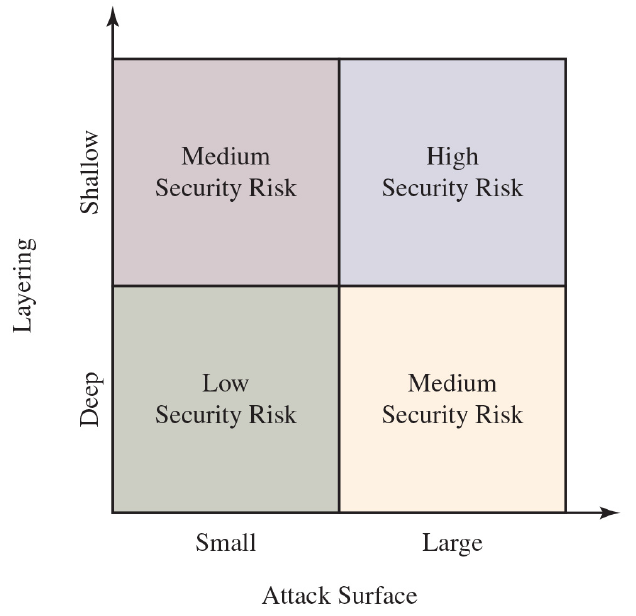
\includegraphics[width=0.5\linewidth]{resources/fig1.png}
        \caption{Defensa en profundidad y Superficie de ataque}
        \label{fig:defensa-profundidad-superficie-ataque}
    \end{figure}

    \section{Estrategia de seguridad informática}
    \begin{itemize}
        \item Política de seguridad: normas, roles y responsabilidades para proteger activos y regular accesos y comportamientos.
        \item Implementación de seguridad:
        \begin{itemize}
            \item Prevención: controles proactivos, endurecimiento y mínimo privilegio.
            \item Detección: monitorización, alertas y registros.
            \item Respuesta: contención, erradicación y comunicación.
            \item Recuperación: restauración, lecciones aprendidas y mejora continua.
        \end{itemize}
    \item Garantía (\textit{assurance}): grado de confianza en que el sistema hace cumplir la política de seguridad bajo condiciones previstas.
    \begin{itemize}
        \item Evidencia: requisitos trazables, diseño, pruebas, resultados de verificación, registros y documentación.
        \item Verificación y validación: revisiones técnicas, análisis estático/dinámico, pruebas unitarias/integración/aceptación.
        \item Gestión de configuración y cambios: control de versiones, líneas base, revisiones, segregación de entornos y firmas.
        \item Criterios y certificación: perfiles de protección, niveles de garantía y evaluaciones independientes.
        \item Métricas y monitorización continua: cobertura de controles, vulnerabilidades, MTTR y eficacia de remediaciones.
    \end{itemize}
    \item Evaluación: examen sistemático de la eficacia de los controles y del riesgo residual.
    \begin{itemize}
        \item Técnicas: escaneo de vulnerabilidades, pruebas de penetración, fuzzing, red/purple teaming y hardening verificado.
        \item Cumplimiento: auditorías frente a políticas y estándares, recopilación de evidencias y gestión de hallazgos.
        \item Seguridad en el ciclo de vida: SAST, DAST, SCA, análisis de IaC y cadena de suministro.
        \item Gestión de riesgos: estimación de impacto/probabilidad, tratamiento y aceptación documentada del riesgo residual.
        \item Mejora continua: lecciones aprendidas, planes de acción, seguimiento y verificación de eficacia.
    \end{itemize}
    \end{itemize}
    \section{Estándares (muy breve)}
    \begin{itemize}
        \item ISO/IEC 27001/27002: SGSI y catálogo de controles para gestión y operación.
        \item NIST SP 800-53 y RMF: controles y gestión del riesgo en sistemas de información.
        \item CIS Controls v8: salvaguardas priorizadas y medibles para higiene básica.
        \item PCI DSS: requisitos para proteger datos de titulares de tarjeta.
        \item OWASP ASVS/Top 10: verificación y prácticas para seguridad de aplicaciones.
        \item SOC 2 (AICPA): criterios de seguridad, disponibilidad, integridad, confidencialidad y privacidad.
    \end{itemize}
    Objetivo: alinear políticas, controles y evidencias para facilitar cumplimiento, auditoría y mejora continua.

\end{document}
